\documentclass{article}

\usepackage[utf8]{inputenc}
\usepackage{graphicx}
\usepackage{url}
\usepackage{color}
\usepackage{titlesec}
\usepackage{amsmath}
\usepackage{physics}
\usepackage{amsfonts}
\usepackage{subcaption}
\usepackage{booktabs}
\graphicspath{{../figures/}}

\title{Declarative proto-paper for supersat project}
\author{K. Latimer}
\date{Nov 17, 2020}

\newcommand{\drcomm}[1]{\textcolor{blue}{\textit{#1}}}
\newcommand{\klcomm}[1]{\textcolor{red}{\textit{#1}}}

\begin{document}

\maketitle

\noindent\drcomm{Questions/comments from DR in blue} \\
\noindent\klcomm{Responses from KL in red}\\

In order to determine experimental supersaturation within a reasonable margin of error, we must use the quasi-steady-state (QSS) supersaturation formula [cite]. Based on our analysis of the WRF data, this approximation is only valid within certain limits, namely:
\begin{itemize}
	\item T \textgreater  273K (we're not including ice in the theory; note that Fan et al do evaluate SS wrt water above the freezing line though)
	\item w \textgreater  2 m/s (reasonably strong updrafts)
	\item cloud LWC \textgreater  1e-4 g/g (in the convection core)
	\item including rain droplets and ventillation corrections
\end{itemize}

Figure \ref{wrfvsqss} shows a scatterplot with the agreement between the actual and QSS-derived SS values in the WRF simulation, for points satisfying the above criteria.

\clearpage
\newpage

\begin{figure}[ht]
	\centering
	\begin{subfigure}{0.7\textwidth}
		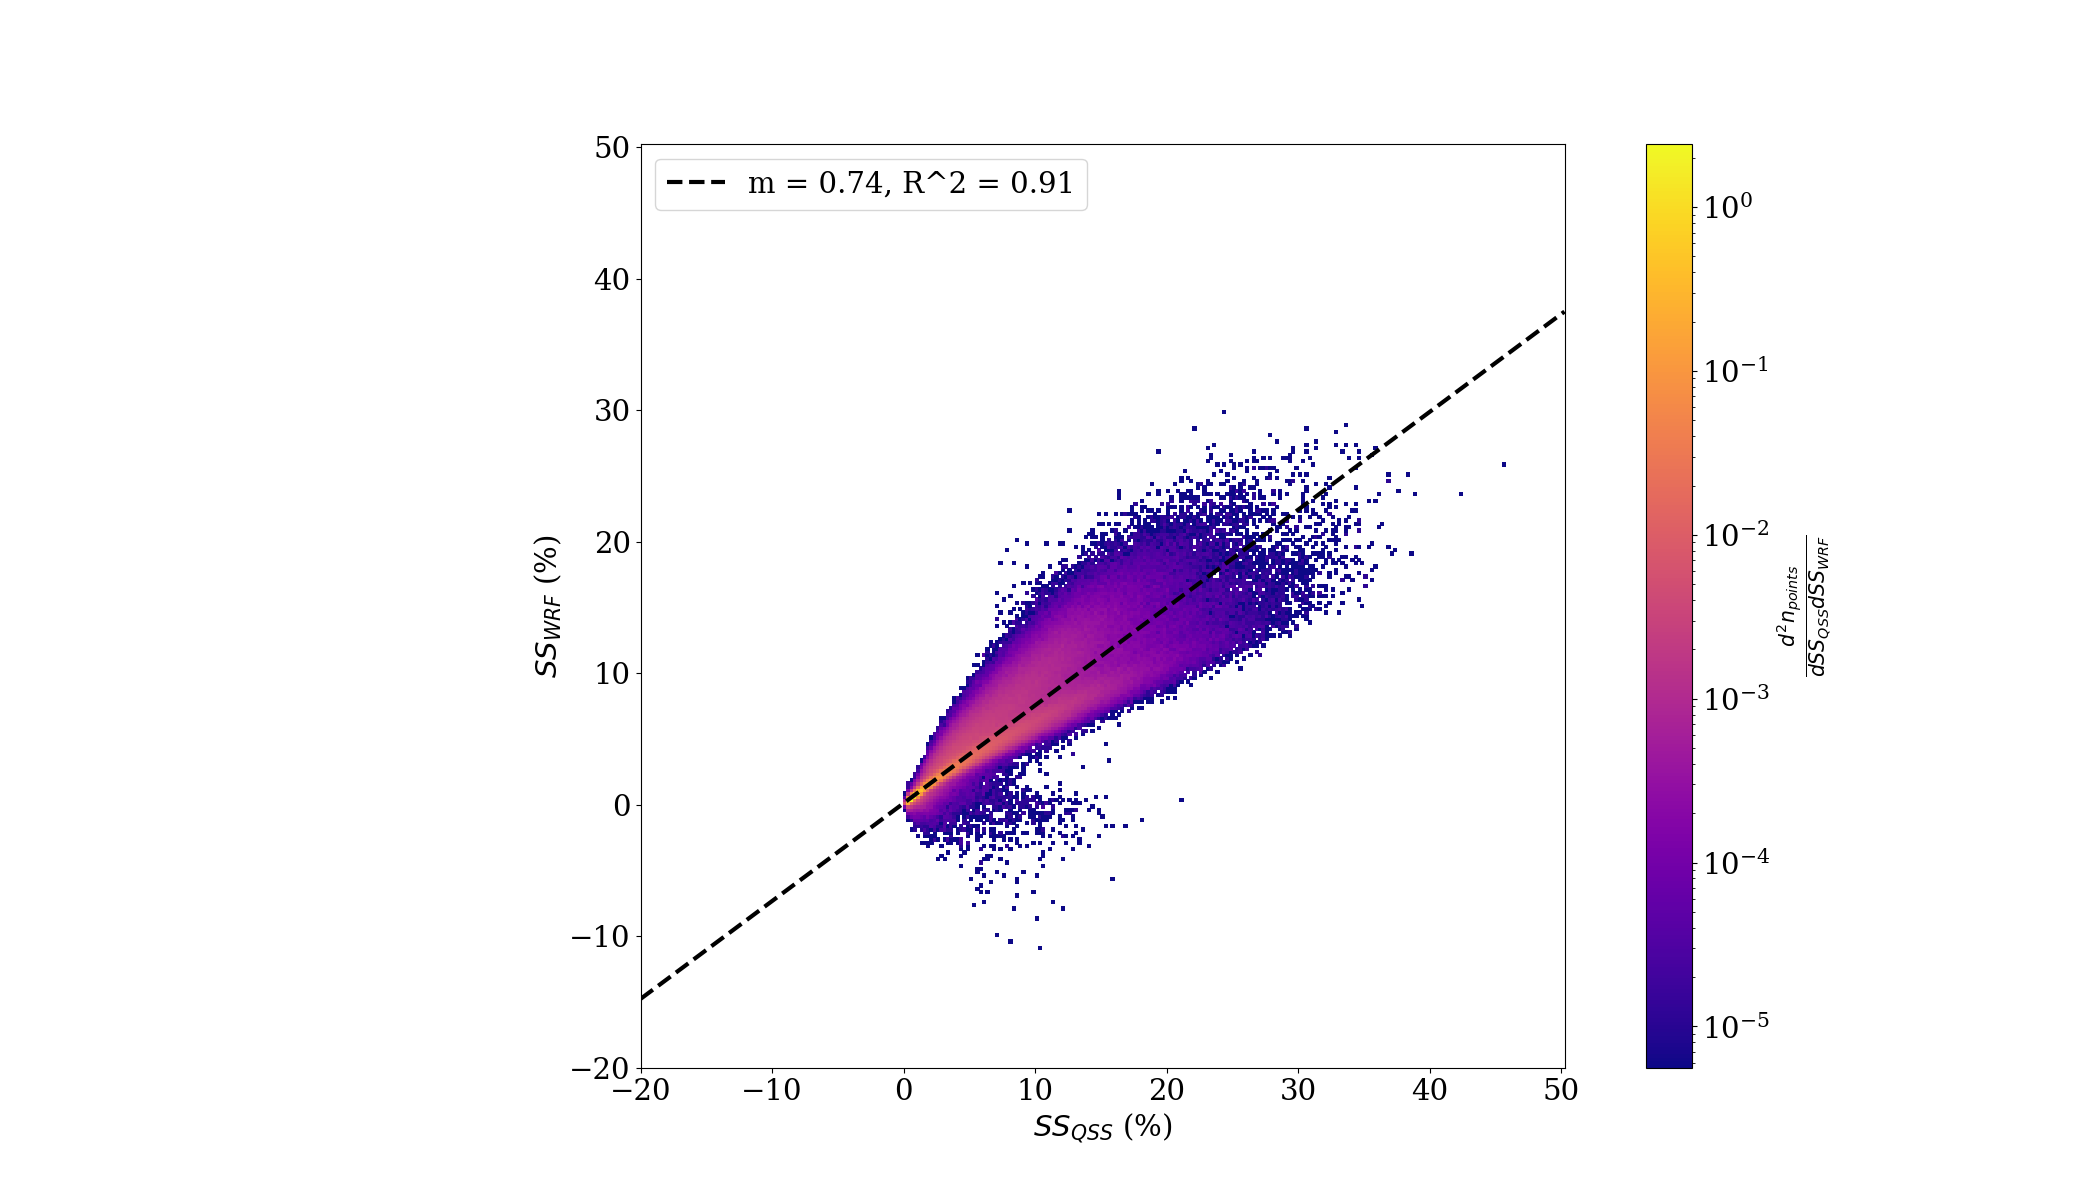
\includegraphics[width=\textwidth]{revmywrf/v12_heatmap_ss_qss_vs_ss_wrf_Unpolluted_figure_6.png}
		\caption{Unpolluted case.}
		\label{wrfvsqssunpoll}
	\end{subfigure}
	\begin{subfigure}{0.7\textwidth}
		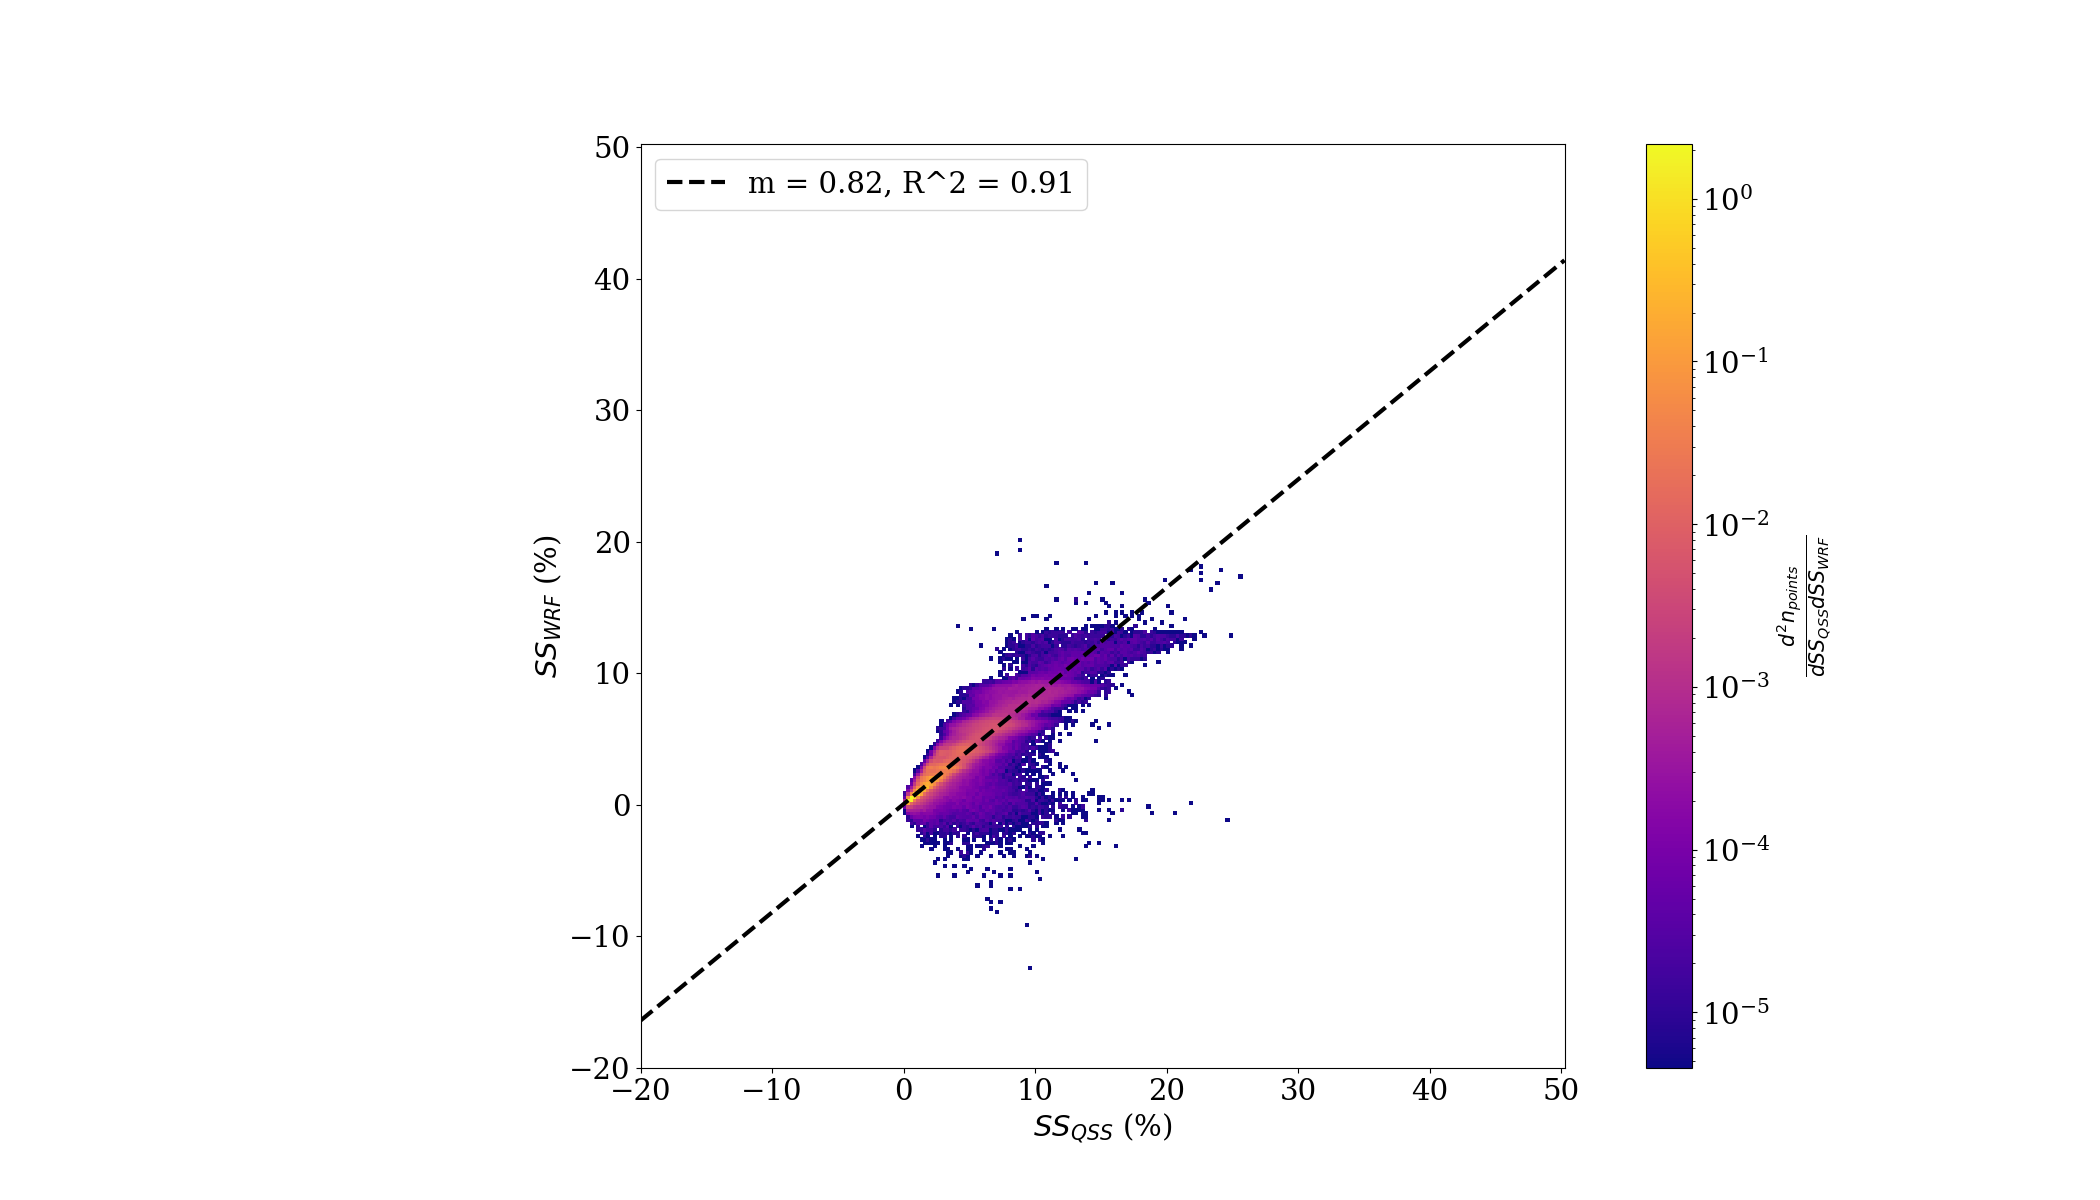
\includegraphics[width=\textwidth]{revmywrf/v12_heatmap_ss_qss_vs_ss_wrf_Polluted_figure_6.png}
		\caption{Polluted case.}
		\label{wrfvsqsspoll}
	\end{subfigure}
	\caption{Actual ($SS_{WRF}$) vs predicted ($SS_{QSS}$) supersaturation. Color indicates density of data points; note the scale is logarithmic.}
	\label{wrfvsqss}
\end{figure}

In Fan 2018, they claim that the so-called warm phase invigoration mechanism (WPIM) is driven by the presence of ultra-fine aerosol particles with sub-50nm diameters (UAP50) on the order of ~1000/ccm (polluted case; contrasted with between 0 and 60/ccm in the unpolluted case) [\drcomm{What different in UAP50 is supposedly fueling the WPIM?} \klcomm{They don't really offer any explanation besides to say that ``the low total aerosol concentration, ultrafine aerosol particles with diameters less than 50 nm are typically nearly absent over the Amazon rainforest, as new particle formation has rarely been observed in the boundary layer there."}] in the boundary layer (BL) where cloud droplets are nucleated. Crucial to this argument is the claim that, without such particles present, the troposphere supports very high supersaturations. In particular, this paper reports average supersaturations in the upper tenth percentile of updrafts in convective cells as high as [\drcomm{``as high as" or on average?} \klcomm{I am referencing the maximum SS values in the vertical profiles in Figure 4 (top two panels) of the paper...I could take the vertical average, but over what altitude range?}] $\approx$ 4 and 15\%, in the warm cloud and deep cloud phases \footnote{After Fan et al 2018, ``Warm cloud" phase: ``30-min duration after the warm rain starts and the rain rate exceeds 0.5 mm/hour"; ``Deep cloud" phase: ``30-min duration with 15 min before and after the strongest convection." [\drcomm{Are you using the same criteria?} \klcomm{Well I think that would require tracking down ground-based precipitation rate measurements, which I have not tried to do. As far as analyzing the WRF data, the only things I'm including in the paper as it stands are the evaluation of the QSS approximation, which doesn't need to be limited to any specific time periods in my mind; and the vertical wind velocity distribution, which I'm comparing directly to the experimental data that, as just stated, are not separated into these cloud phases right now.}]}, respectively, from WRF simulations of the pristine, pre-industrial Amazon rainforest. By contrast, the highest simulated supersaturations under typical modern-day pollution levels as observed in simulations were $\approx$ 1 and 6\%, respectively. 

In order to get a feel for how O(10\%) supersaturation would affect the energetics of a rising parcel of air relative to one with O(1\%) supersaturation, we estimate the difference in convective available potential energy (CAPE) between the two over the course of ascent. Assuming no heat of condensation is lost to the environment we have:
\begin{equation}
\label{energyconsv}
C_{ap}dT + L_vdq_v = 0,
\end{equation}
where $q_v$ is the water vapor mass fraction of the parcel ($q_v=m_v/m_{tot}$), also expressed in terms of the the relative humidity ($RH$) and saturation water vapor mass fraction ($q_v^*$) as:
\begin{equation}
\label{qveqn}
q_v = RHq_v^*
\end{equation}
Usig the Clausius-Clayperon equation:
\begin{align}
\label{clauclay}
dq_v^* &= d\Big(\frac{e_sV}{R_vTm_{tot}}\Big)\nonumber\\
&=\frac{de_s}{e_s}q_v^* - \frac{dT}{T}q_v^*\nonumber\\
&=\frac{L_vdT}{R_vT^2}q_v^* - \frac{dT}{T}q_v^*\nonumber\\
&=\Big(\frac{L_v}{R_vT} - 1\Big)\frac{dT}{T}q_v^*\nonumber\\
&\approx \frac{q_v^*L_v}{R_vT^2}dT
\end{align}
Taking the differential of Equation \ref{qveqn} and rearranging terms in Equations \ref{energyconsv}, \ref{qveqn}, and \ref{clauclay} yields:
\begin{equation}
dT = \frac{-L_vq_v^*}{C_{pa} + q_v\frac{L_v^2}{R_vT^2}}dRH
\end{equation}
Plugging in typical values for $RH$ and $T$ gives $dT\approx 0.5K$. We suppose for the sake of this order-of-magnitude estimate that the difference in buoyancy between the two parcels is constant over a length scale of the troposphere's scale height (Is this a correct statement of the reasoning?? I am not sure if I understand why that is valid). Therefore the difference in CAPE is:
\begin{align}
dCAPE &\approx Hg \frac{dT}{T}\nonumber\\
&=Hg\frac{-L_vq_v^*}{T(C_{pa} + q_v\frac{L_v^2}{R_vT^2})}dRH\nonumber\\
&\approx 200 J/kg
\end{align}

We now seek to determine whether such high values actually occur in nature. First we look at data from the ACRIDICON-CHUVA mission (part of the HALO campaign) in the Amazon forest in Brazil. Aerosol concentrations in the BL (ie from ground-based measurements) both upwind and downwind of anthropogenic pollution sources on select [\drcomm{Spell out what criterion was used to ``select" flight dates.} \klcomm{To be honest this was really just a schematic placeholder while I'm still waiting on the ATTO data...since there was a large degree of variability between dates (and also within single dates over the course of time) it didn't seem right to average over all of them. Maybe in the final version I should just put all dozen or so of them in a single figure in their own panels?}] flight dates are shown in Figures \ref{attoasd} and \ref{goaasd}, respectively.

\clearpage
\newpage

\begin{figure}[ht]
    \centering
    \includegraphics[width=9cm]{atto/atto_psd_figure.png}
    \caption{[DON'T HAVE DATA YET] Aerosol particle size distribution for a representative date; ground-based measurement coinciding with ACRIDICON-CHUVA flight dates, compared to initial distribution in boundary layer for WRF simulation. From ATTO site, upwind of Manaus metropolitan area.}
    \label{attoasd}
\end{figure}
\begin{figure}[ht]
    \centering
    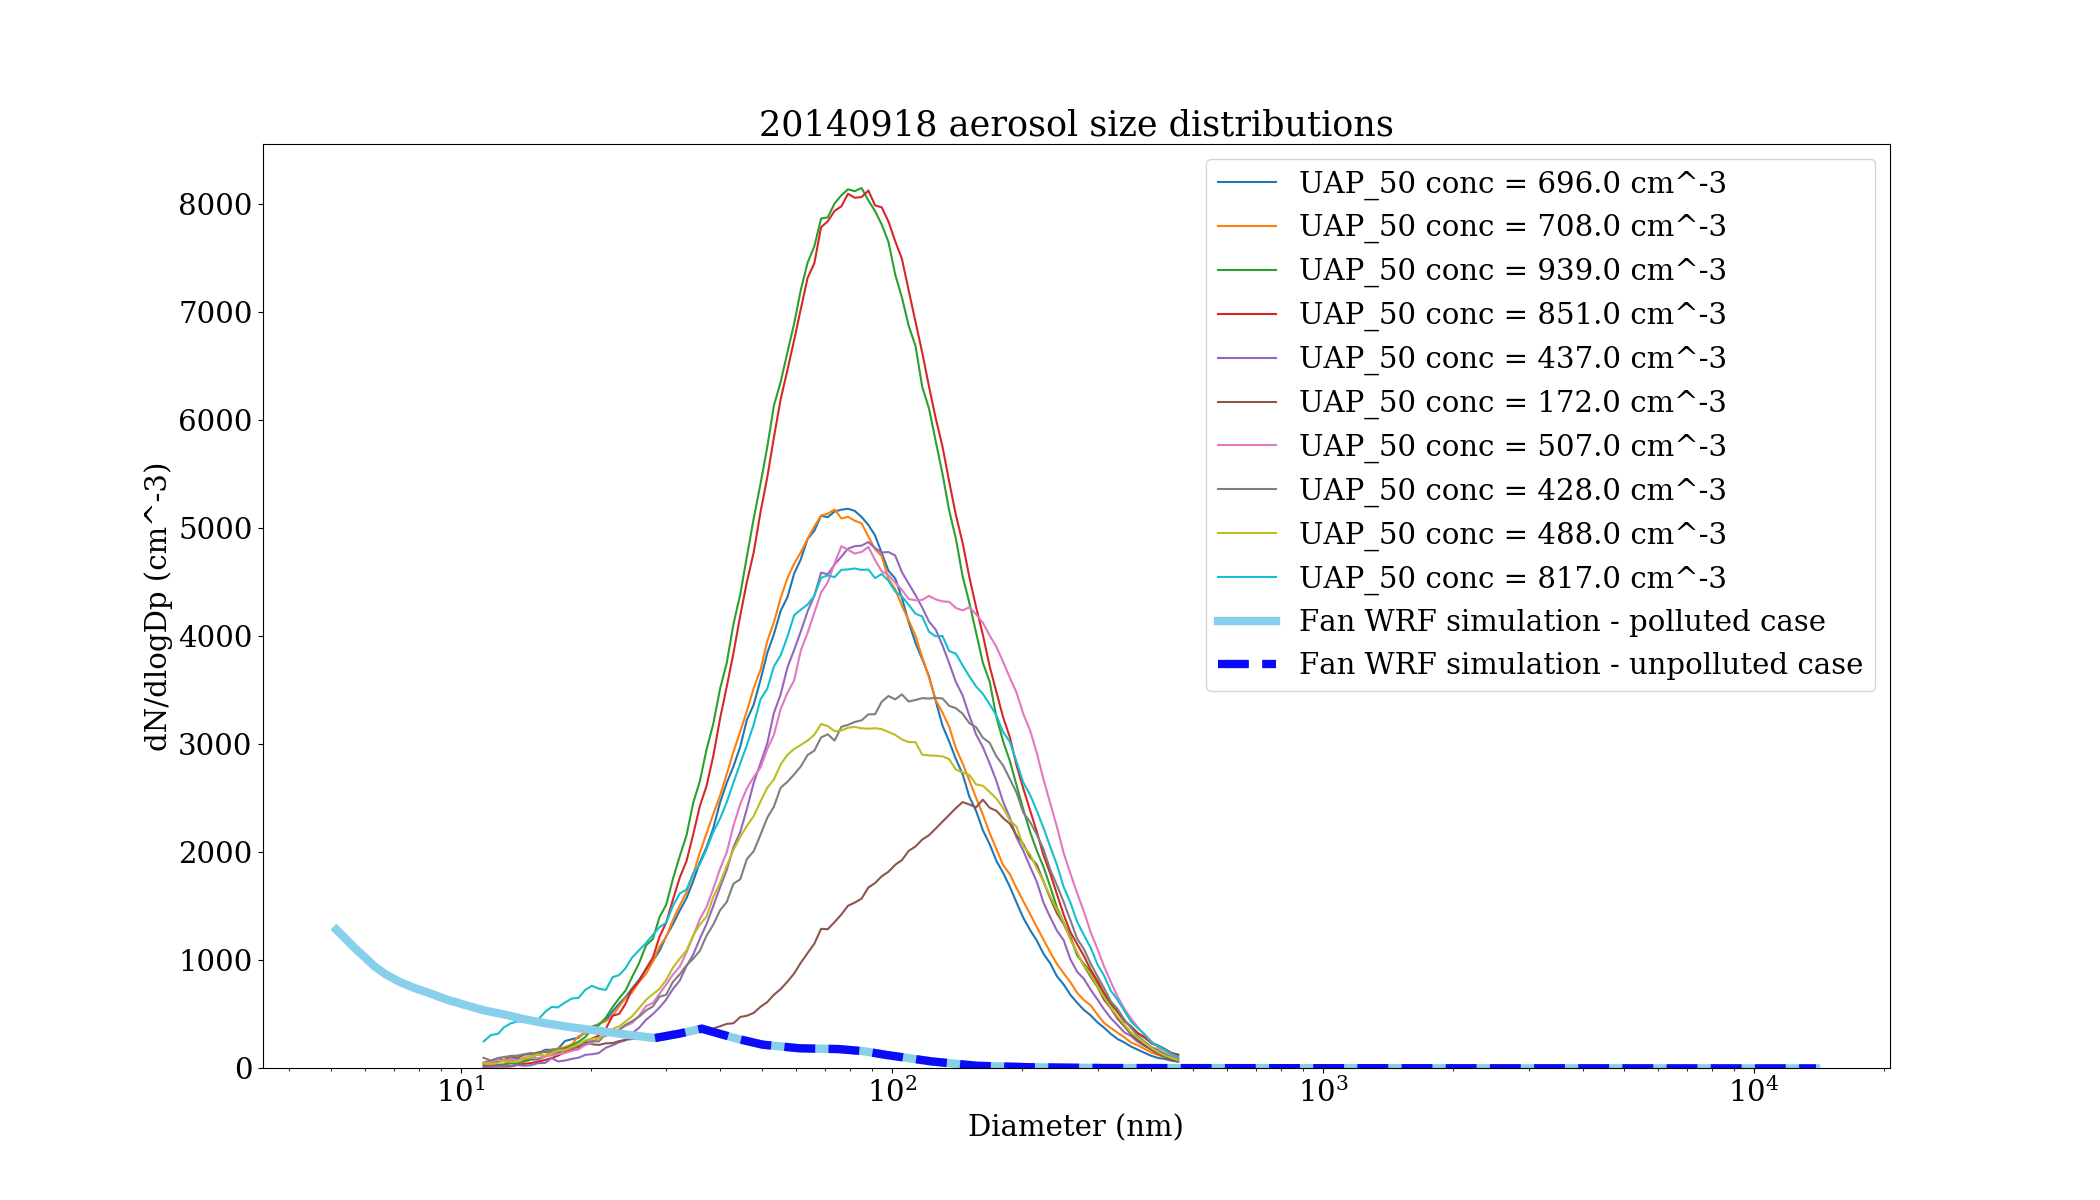
\includegraphics[width=12cm]{goama/v6_aero_size_distb_20140918_figure.png}
    \caption{Aerosol particle size distribution for a representative date; ground-based measurement coinciding with ACRIDICON-CHUVA flight dates, compared to initial distribution in boundary layer for WRF simulation. Curves represent the average over $\approx$2-hour samples. From GoAmazon site, downwind [\drcomm{Were there no upwind aerosol measurements? I would think there must have been, as that upwind/downwind aerosol difference was the rationale for GoAmazon. Is that Mira Pohlker's data? If so, I am surprised DOE did not set up measurements that would be availbe in the ARM archive.} \klcomm{Yes, this is what I'm still waiting on from Pohlker. Have looked through the ARM archive's GoAmazon datasets and can't find it; nor are the measurements I'm looking for hosted on the separate ATTO online database.}] of Manaus metropolitan area.}
    \label{goaasd}
\end{figure}

[\klcomment{Realized my initial wording here was incorrect / vague}] Even though UAP50 levels in the BL approach (from above) the upper bound of what Fan et al used in their simulations of the unpolluted pre-industrial conditions (??? pending ATTO measurements from Mira Pohlker), we do not find any supersaturation values in the troposphere exceeding 1\% using the criteria above (Figure \ref{haloqsshist}). The average value of $SS_{QSS}$ measured at all points satisfying the above filtering criteria is 0.23\% (std. dev. 0.15\%) [\drcomm{Compared to what from Fan et al.?} \klcomm{I think making this comparison requires revisiting the whole ``warm cloud / deep cloud" filtering scheme...feeling like I'm at the point where I just need to discuss this in person to figure out what makes sense.}]. Of those points, we find the average $SS_{QSS}$ for the top tenth percentile of updrafts (as measured by vertical wind velocity) is 0.32\% (std. dev. 0.18\%). [NOTE: Need to do quantitative error analysis on these data] [\drcomm{Of what kind and to make what point? The conclusion already seems clear.} \klcomm{I just figured that was good practice but if you don't think it's necessary I will happily cross it off the list.}]

\clearpage
\newpage

\begin{figure}[ht]
    \centering
    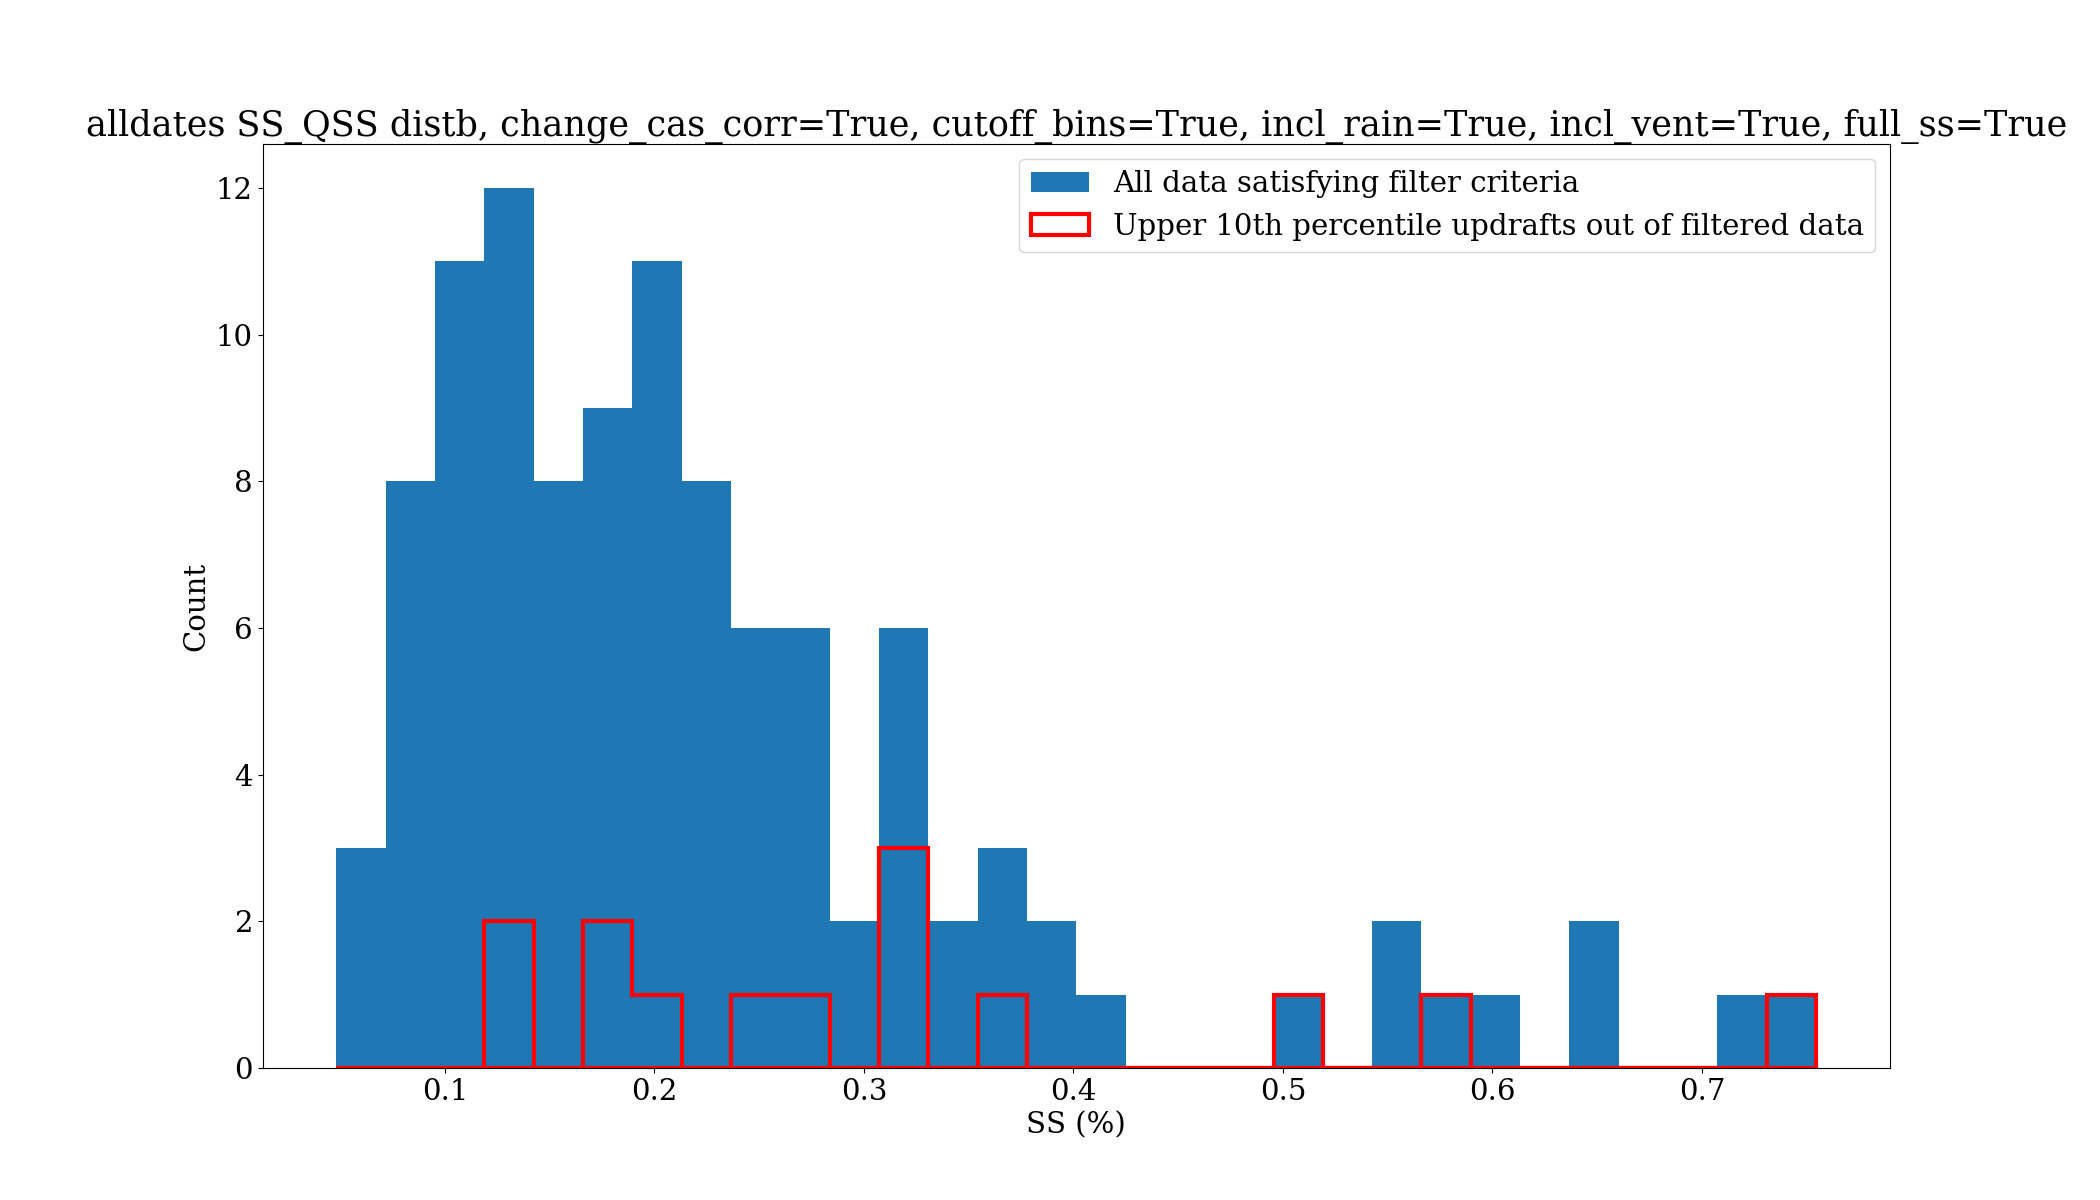
\includegraphics[width=9cm]{revhalo/v24_with_up10perc_ss_qss_hist_cas_alldates_figure.png}
    \caption{Predicted ($SS_{QSS}$) supersaturation distribution from HALO field campaign (all flight dates). Using filtering criteria outlined in the text. Overlying histogram in red is the distribution for points lying in the upper tenth percentile of updrafts (as measured by vertical wind velocity), after Fan 2018.}
    \label{haloqsshist}
\end{figure}

Next we look at data from the CAIPEEX experiment in India. No ground-based aerosol concentration measurements are available (and measurements in the troposphere from instruments on the plane are sketchy...). Supersaturation distribution using the same criteria is shown (for all flight dates combined) in Figure \ref{caipeexqsshist}. We see a relatively small number of supersaturation values exceeding 1\%. The average value of $SS_{QSS}$ measured at all points satisfying the above filtering criteria is 0.49\% (std. dev. 0.64\%). Of those points, we find the average $SS_{QSS}$ for the top tenth percentile of updrafts (as measured by vertical wind velocity) is 0.90\% (std. dev. 0.96\%). [NOTE: Need to do quantitative error analysis on these data]

\begin{figure}[ht]
    \centering
    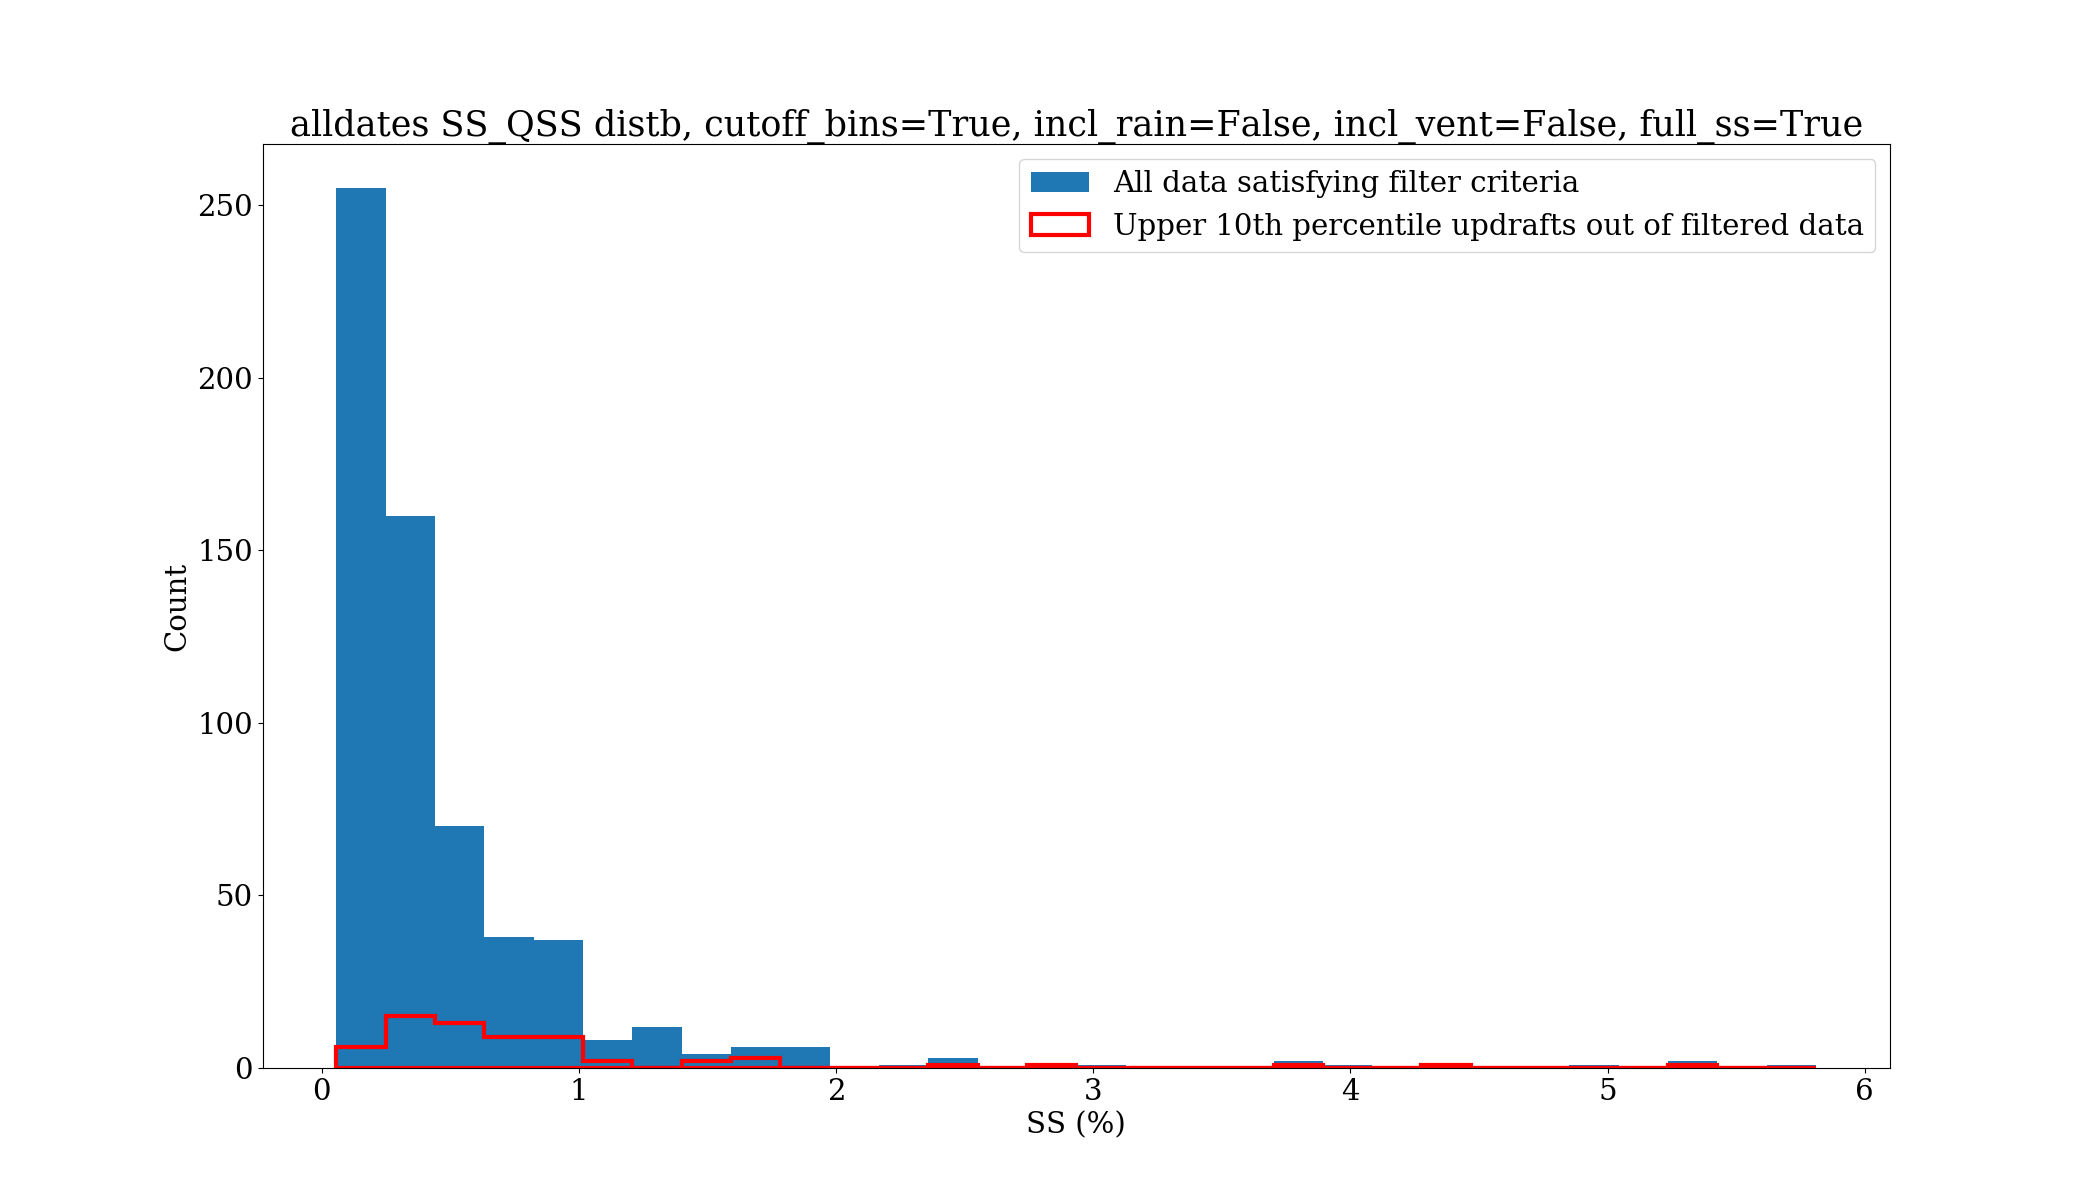
\includegraphics[width=9cm]{revcaipeex/v10_with_up10perc_ss_qss_hist_alldates_figure.png}
    \caption{Predicted ($SS_{QSS}$) supersaturation distribution from CAIPEEX field campaign (all flight dates). Using filtering criteria outlined in the text, but not including rain drops or ventilation corrections due to lack of data. Overlying histogram in red is the distribution for points lying in the upper tenth percentile of updrafts (as measured by vertical wind velocity), after Fan 2018.}
    \label{caipeexqsshist}
\end{figure}

Conclusion: Fan gets a difference in supersaturation (between polluted and clean) of 5\% (11\%) for the warm (deep) cloud phase (averaged over the top tenth percentile of convective updrafts), which supports 100 J/kg (200 J/kg) of invigoration in the polluted case. Here, we find average supersaturations in the top tenth percentile of convective updrafts to be 0.9\% and 0.3\% in CAIPEEX and HALO, respectively, which would support only $\approx$ 10 J/kg [\klcomm{managed to lose track of a factor of ten somewhere!}] invigoration relative to a storm with zero supersaturation [Note this argument is still somewhat contingent on better aerosol data esp. from the ATTO experiment...could just be we are only looking at polluted environments in these field campaigns]. 

One possible counterargument is that the flight campaigns simply didn't fly through strong enough updrafts. However the vertical velocity distributions from the campaigns are quite similar to that from the simulations. See Figure \ref{combinedwhist}. 

\begin{figure}[ht]
    \centering
    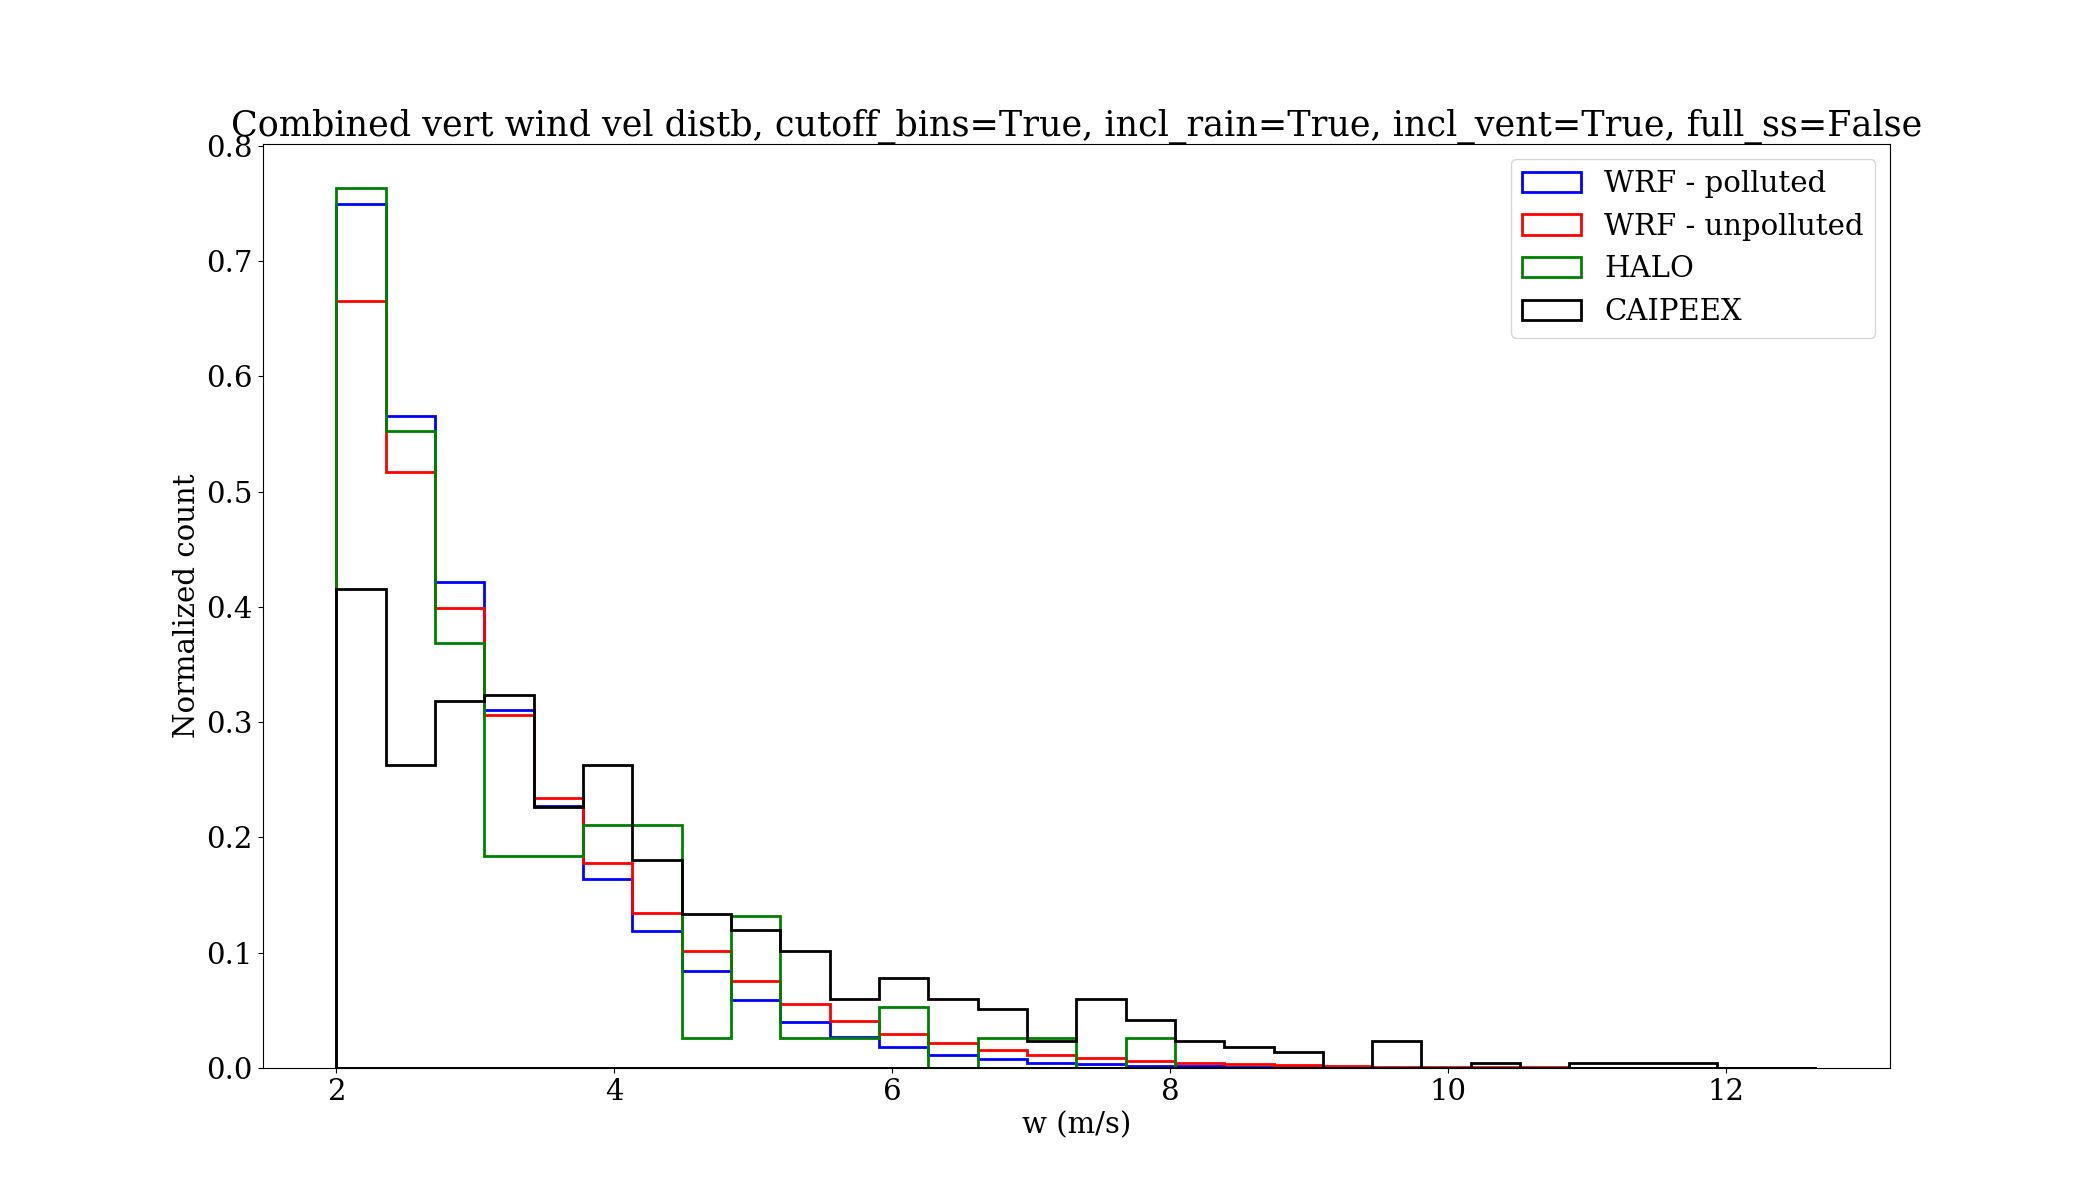
\includegraphics[width=12cm]{revmywrf/v9_combined_w_hist_figure.png}
    \caption{Vertical wind velocity distribution from simulations and field campaigns. Using filtering criteria outlined in the text.}
    \label{combinedwhist}
\end{figure}

\end{document}
